\chapter{Data Productions}

\red{CHAPTER STATUS: IN PROGRESS}

During my tenure at SeaQuest, I was primarily in charge of the effort to decode the raw, serialized data from the data acquisition systems and store it in a manner in which it could be readily accessible by collaborators worldwide. Beyond that, emphasis was placed on curating the tracked physics data and preparing it in such a way that facilitates quick and simple analysis from many different analytical software packages.

The technologies used to perform this were a combination of compiled C/C++ codes, MySQL, ROOT, and the Fermilab Computing Division's primary computing grid. The end product provided to all collaborators was in the form of unified MySQL database ``schemas'' (or, groups of tables) possessing all of the combined run, spill, event, slow control, and tracked information, along with specific data quality flags in place to assist in the selection of good analysis data.

\section{Raw Data Processing}

The three raw outputs of the data acquisition systems, as described above (and in Chapter 2) are Main DAQ CODA files, Scaler DAQ CODA files, and Beam DAQ ASCII files. Each raw data file corresponds to the data taken from certain subsystems over approximately one to two hours of running time. These three types require varying degrees of de-serialization, parsing, processing, and storage -- a process as a whole defined as \emph{decoding}. 

All raw data files are backed up to long-term tape storage (managed by FNAL Computing Division), and the decoded and processed data gets stored on one of four MySQL servers to be used for analysis by the collaboration. Data is also output to ROOT files for ease of use by independent tracking programs.

\subsection{CODA Event Format}

A single CODA file can be described as being a chain of events. These can generally be divided into ``CODA Events'' for those related to the CODA file itself, and ``Standard Physics Events'' when containing experimental data read out by CODA and its subsystems. Each event can be represented by an array of unsigned 32-bit integers. When using the CODA EVIO (event input/output), one whole event is read out into such an array, which can vary in size from 6 to $\sim50,000$ integers long, depending on the type of content.

CODA Events primarily correspond to the actions taken by a shift-taker using the \emph{rcgui} application on the data acquisition computer. The types of events that fall under this category are: Sync, Prestart, Go, Pause, and End. It should be noted that the Sync and Pause events do not generally get used at SeaQuest. These provide markers in the CODA file of what commands were given to CODA through the course of taking data. 

Before data taking can begin The readout controllers and the trigger supervisor need to be loaded with a designated firmware in order to operate properly. Before a CODA file is started and created, this ``Download'' is performed, and then CODA is ready to transition from the downloaded state to the prestarted state. The CODA file is then initialized with a prestart event, whose format can be seen in Figure~\ref{fig:coda-prestart-go}. The most important information stored in the prestart event is the run number, which is used universally through the experiment. 

Once in a prestarted state, a ``Go'' action is initiated to transition it into data taking mode. This action generates a Go event. If ever paused, a Go event would be created once data taking was resumed. Go events contain the current time and the number of events in the run so far, also seen in Figure~\ref{fig:coda-prestart-go}. It should be noted that the ``time'' stored in these events is not trusted, as the data acquisition computers are not synced to an official external source.

\begin{figure}
	\centerline{
		\mbox{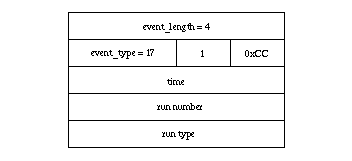
\includegraphics[width=0.5\textwidth]{figures/production/prestart_event.png} 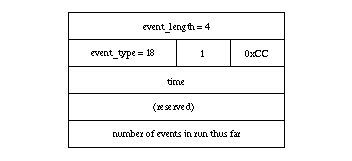
\includegraphics[width=0.5\textwidth]{figures/production/go_event.png}}
	}
	\caption{(Left) The Prestart event, with event type 17; (Right) The Go event, with event type 18\cite{jlab:coda}.}
	\label{fig:coda-prestart-go}
\end{figure}

The last CODA Event of importance is the End Event. This contains the number of events in the run, but primarily serves as a marker to any programs reading the CODA file that the EOF (end of file) has been reached, and to commence any post-run processes.

Most of the events in the CODA file, however, will be ``Standard Physics Events''. The contents of these can be varied, but can be characterized generally as having a header containing the total length of the event (in number of 32-bit integer ``data words''), followed by several ``data banks'', which are typically filled with a series of ROC outputs (Fig.~\ref{fig:coda-physics-roc}). The contents and formats of the ROC data banks are completely controlled by the ROC programming, and whatever set of 32-bit words the ROC has to read out, it will store in its ``data words'' block. 

\begin{figure}
	\centerline{
		\mbox{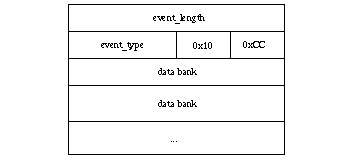
\includegraphics[width=0.5\textwidth]{figures/production/physics_event.png} 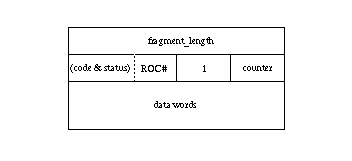
\includegraphics[width=0.5\textwidth]{figures/production/roc_event.png}}
	}
	\caption{(Left) A standard physics event, with various event types, filled with a series of data banks; (Right) The ROC data bank format\cite{jlab:coda}.}
	\label{fig:coda-physics-roc}
\end{figure}

\subsection{ROC Data Bank Formats}



\subsection{Decoding Raw Data}

The CODA file decoding process is nearly identical in the cases of the Main DAQ and Scaler DAQ outputs, and only differ by content; the Scaler DAQ reads out specific scaler data, and the MainDAQ contains TDC readouts of the detectors. For each one to two hour \emph{Run}, the CODA files can be well-described as the following sequence of events (and the data they contain):
\begin{enumerate}
	\item Prestart Event (Run data)
	\item Begin Spill Event (Spill data, Scaler readout)
	\item Many Physics Events (Event data, TDC readout)
	\item End Spill Event (Spill data, Scaler readout)
	\item SlowControl Event (Slow control readout, Spill ID readout)
	\item Spill Counter Event (Spill ID readout) \newline ...(Repeat 2-6 for each \emph{Spill})
\end{enumerate}

The decoding programs use C and C++ in conjunction with Jefferson Lab's CODA I/O library\cite{jlab:coda} to read these events and parse them according to their individual formats. Data from these CODA events are decoded and placed into hierarchical categories.

\subsubsection{Run Level Data}

Run-level data contains data and metadata pertaining to the entirety of the run that is recorded. At the time of the Prestart Event, the date and time of the run are stored, along with a readout of the specific settings of all non-trigger TDC boards. Settings regarding which triggers are enabled and what each of their prescale factors is also stored in the run-level data.

After the End Event is encountered, metadata is aggregated and stored regarding such items as the number of chamber hits, the types of triggers that were fired, the target positions used, average magnet currents, and other useful metrics. All of these fields of settings and aggregated values can be used later on to quickly determine if a run is analyzable, or if it has characteristics that are desirable for specific niche analyses.

\subsubsection{Spill Level Data}
The \emph{Beginning of Spill} (BOS) and \emph{End of Spill} (EOS) events bookend the set of physics events for a given spill. At each BOS and EOS events, the 140 MHz VME scalers are read out. At the beginning of the spill, all scalers are zeroed out, and then read out again after the spill has ended.

Slow Control events are read out between spills, which contain data regarding the current spill identifier number, target systems, beam and radiation monitors, and environmental readings.

The spill identifier (\emph{spillID}) is what is used to synchronize the data together across various data acquisition systems. As such, the \emph{spillID} is read out redundantly in both Slow Control and Spill Counter events (which contain only the \emph{spillID} value) to ensure that the data is appropriately labeled.

When the End Event (for the whole CODA file) is reached, the independently-recorded Beam DAQ data (recorded in an ASCII file) is read and stored with the rest of the Spill-level data.

\subsubsection{Event Level Data}
For each spill, $\sim3k$ events are triggered to be recorded, though this number can vary greatly with the particular beam settings of a run. With each event, three types of information is stored: the trigger which fired the event, a measure of the beam intensity per RF bucket, and the full detector readouts. The detector readouts require the most processing of all the rest of the data. The CODA files contain the hardware addresses of each detector \emph{hit}, along with a \emph{TDC time}. The following steps briefly summarize the processing steps:
\begin{enumerate}
	\item Mapping: Map the hardware address to a detector name and detector element number
	\item Timing: Classify hits as in-time or not and calculate \emph{drift time} from TDC time
	\item R-T (time-to-space): Translate \emph{drift time} to \emph{drift distance}
	\item After-Pulse Elimination: Remove hits that result from signal reflection and other electronic artefacts
	\item Trigger Road Reconstruction: Use \emph{v1495} TDC hits to reconstruct possible trigger roads that may have fired
	\item Hodoscope Masking: Remove drift chamber hits that have no adjacent hodoscope hit
	\item Trigger Road Masking: Same as hodoscope masking, but only using hodoscopes from reconstructed trigger roads
\end{enumerate}
This fully processed data is then stored into one the experiment's MySQL databases and/or a ROOT file.

%%%%%%%%%%%%%%%%

\section{Online and Offline Processing}

There are two running modes of raw data processing: on-line and off-line. For on-line mode of productions, all Run- and Spill-level data is decoded, but only 1-in-$n$ Physics Events are processed, where $n$ is typically between 3 and 15, depending on the event data taking rates. This \emph{``sampling mode''} is used in order for the decoding to reliably keep up with even high-intensity beam data. This data pipeline is important for on-line monitoring of the experiment by shift crews. With this up-to-the-minute stream of data, any abnormalities in duty factor, wire maps, et al. can be observed directly and acted upon quickly.

For off-line, or ``batch'', productions, a large group of categorically similar runs is defined, and the chain of production processing is initiated. The steps of this process is generally emph{decoding, tracking, archiving, and merging}. The logical blocks of runs are typically defined by ``roadset'', or, the version of the set of trigger roads used in the L1 trigger matrix. Differences in these trigger matrices can affect the distributions to a degree commensurate with the difference in the set of roads that are triggered on by the FPGA-1 trigger. As such, each block of data using a given roadset should be analyzed individually and then have its results combined with those of other roadsets via a weighted average.

The decoding and tracking is performed on Fermilab Computing Service's FermiGrid, which provides the computing resources necessary to process hundreds of runs simultaneously. The tracking has also expanded its capabilities to run on the Open Science Grid, which is a grid computing network that pools together computational resources from national laboratories and universities throughout the world\cite{osg:doc}. This allows the intensive reconstruction algorithms to perform its tracking on thousands of grid nodes at once.

A single decoding job submission will output the processed data to one of the four available MySQL servers and also to a ROOT file. The processed data in ROOT form at this stage is called the ``digit'' data. Whether or not the decoding sends Hit and TriggerHit information to the MySQL schemas is an option that can be set at the time of batch processing. The current operating mode is to perform batch processing, sending Hit/TriggerHit data to MySQL for only 1-in-50 runs. This allows users to capture a glimpse of full hit distributions for runs within a roadset while preventing a single pass of the experiment's data from filling up all available data storage space.

After this step, jobs will be submitted to run one or both of the two tracking programs based on the ROOT file and/or the MySQL data. Once the tracking is completed, the ROOT file is archived on the Fermilab BlueArc NAS backup system for storage and for tracking.

Upon the completion of decoding and tracking of a specified range of runs, all of their Run-, Spill-, and Event-level data, along with its tracked data, is combined into a single \emph{merged} schema. These \emph{merged} schemas are mirrored across all four of the MySQL servers for optimal redundancy and availability.

\section{RDBMS Data Structure}

The processed data is primarily stored in MySQL Server 5.1 databases. MySQL is an open-source \textbf{R}elational \textbf{D}ata\textbf{b}ase \textbf{M}anagement \textbf{S}ystem (RDBMS) developed by Oracle that is well-suited for the storage and responsive querying of hierarchical data.

Each run is decoded into its own schema, and contains its own instances of all tables of a specified design. The tables are all \emph{join}-able to each other by sharing \emph{foreign keys} with each other in the form of the \emph{runID}'s, \emph{spillID}'s, and \emph{eventID}'s. The contents of the tables are \emph{indexed} in such a way that \emph{joins} and queries gain a speed performance boost, but this comes at the cost of disk space.

The data on the server is world-wide accessible and can be queried using the standard querying language. The queried data can be directed to any analysis code in any programming language due to the large array of MySQL API's available.

\section{Data Quality}

